\section{Fabrication}

\subsection{Overview}
\paragraph*{}
Questions to answer:
\begin{itemize}
\item N-well or P-well?
\item Will Au work or do we need to use Pt? Schottky effect concerns?
\item Design modified RCA clean for oxide stripping? Just an HF dip?
\item Do we want to use Emulsitone #187 with positive photoresist? Glass forming solution seems to be OK from docs.
\end{itemize}

\subsection{Budget}
\subsubsection{Chemicals}
\newcolumntype{R}{>{\raggedleft\arraybackslash}r}%
\begin{tabularx}{\linewidth}{|X|R|}
\hline {\bf Item} & {\bf Price} \\ 
\hline Acetone, $>99\%$, 950 mL & \$7.95 \\ 
\hline Isopropanol, $>99\%$, 950 mL & \$8.95 \\ 
\hline Distilled water & ?? \\ 
\hline 3\% HF (Whink rust remover), 10 oz & \$3.88 \\ 
\hline SP24 positive photoresist, 8 oz & \$120.04\\
\hline Colloidal silica for CMP, 16 oz & \$29.95 \\ 
\hline Emulsitone Borosilicafilm, 4 oz & \$250.00 \\
\hline Emulsitone Phosphosilicafilm, 4 oz & \$250.00 \\
\hline Emulsitone \#122 Glass Forming Solution, 4 oz& \$250.00 \\
\hline Emulsitone Goldfilm, 4 oz & \$400.00 \\
\hline 
\end{tabularx} 
\subsubsection{CMP polisher parts}
\subsubsection{Spin coater parts}
\subsubsection{Stepper parts}
\subsubsection{Other tools}
\begin{tabularx}{\linewidth}{|X|R|}
\hline {\bf Item} & {\bf Price} \\ 
\hline Hot plate & ?? \\ 
\hline Oven & \$525.00 \\ 
\hline Furnace & ?? \\ 
\hline 
\end{tabularx} 

\subsection{Tooling}

\subsubsection{CMP polisher}

\subsubsection{Furnace}

\subsubsection{I-line mask aligner}
\paragraph*{}
\begin{itemize}
\item Reticle size: 8.5 x 11 inch (215 x 279 mm)
\item Reticle material: transparency film
\item Exposure source: 2x 10W blacklight-blue lamp
\item Reduction factor: 10x
\item Maximum die size: 0.85 x 1.1 inch (21.5 x 27.9 mm)
\item Number of max-size dies on 4" wafer: 7
\end{itemize}
\paragraph*{}
Figure out how to line up the mask with the wafer. Needs a digital timer for precise process control.

\subsubsection{Oven}
\paragraph*{}
Not easy to build, can be purchased prebuilt at reasonable prices.

\subsubsection{Spin coater}
\paragraph*{}
A spin coater was built from several easily available parts:
\begin{itemize}
\item Electric drill
\item Flexible extension
\item Sanding pad
\item 2x4
\item Glass bell jar from outdoor candle holder
\end{itemize}

\paragraph*{}
The current unit works well, and produced very even 3-micron films except for a slight edge ring in tests. However, the lack of
a digital tachometer or feedback system prevents precise process control. It may be advisable to correct this in the future.

\subsection{Processes}

\subsubsection{Spin coating}
\begin{enumerate}
\item Clean spin coater chuck with a paper towel and acetone, rinse with 90\% isopropanol. Air dry.
\item Apply X of masking tape, sticky side up, to spin coater chuck. Tape ends of X to underside of chuck with masking tape.
\item Place wafer on spin coater chuck and press down lightly around edges.
\item If wafer is new (not partially processed), clean with paper towel and acetone, rinse with 90\% isopropanol. Air dry.
\item Use a clean syringe to apply a puddle of coating material to center of wafer. 
\item Wait several seconds for coating to spread.
\item Quickly accelerate to operating speed and hold steady for the required time, then spin down slowly.
\end{enumerate}

\subsubsection{CMP}
Design a chemical-mechanical planarization process using 50nm colloidal silica.

\subsubsection{Photolithography}
\paragraph*{}
This procedure must be performed in low-UV conditions, ideally yellow safelight.
\begin{enumerate}
\item Spin-coat 1mL of photoresist for 45 sec at medium speed (2500 RPM)
\item Bake wafer for 15 minutes at 55 C.
\item TODO: exposure procedure
\item TODO: developing procedure
\item Etching procedures vary by substrate.
\item To strip mask after etching, submerge wafer in acetone bath for 10 sec while gently agitating, then remove and air dry.
\end{enumerate}

\subsubsection{SiO2 deposition}
\begin{enumerate}
\item Spin-coat 1mL of Emulsitone \#122 Glass Forming Solution for 45 sec at medium speed (2500 RPM).
\item Bake wafer for 1 hour at 350 C.
\end{enumerate}
TODO: measure and describe characteristics of typical film, adjust process parameters accordingly. Manufacturer documentation
suggests thicknesses of $1 \mu m$ are typical.

\subsubsection{SiO2 etching}
\begin{enumerate}
\item Preheat hot plate to 150 C.
\item Fill plastic etch tank with 3\% HF solution to 1 cm depth, place on hot plate.
\item Fill plastic rinse tank with distilled water to 1 cm depth.
\item Wait for solution to reach 70 C.
\item Submerge wafer in tank (TODO: design carrier of some sort) and etch 30 sec. TODO: run tests and adjust etch time.
\item Remove wafer and rinse in distilled water. Air dry.
\end{enumerate}

\subsubsection{Doping}
\begin{enumerate}
\item Spin-coat three to four drops of Emulsitone Borosilicafilm or Phosphosilicafilm dopant solution for 15 sec at medium
speed (2500 RPM).
\item Bake wafer for 30 minutes at 80 C.
\item TODO: if we aren't using nitrogen atmosphere, it may be necessary to lay down an un-doped $SiO_2$ layer and planarize.
\item Apply photomask using {\bf positive} of dopant pattern, etch as with standard $SiO_2$ films, strip.
\item Heat wafer for 15 minutes at 1200 C.
\end{enumerate}

\subsubsection{Metal deposition}
\begin{enumerate}
\item Spin-coat 1mL of Emulsitone Goldfilm for 45 sec at low speed (1000 RPM).
\item Heat wafer for 10 minutes at 300 C.
\end{enumerate}
TODO: measure and describe characteristics of typical film, adjust process parameters accordingly. Manufacturer documentation
suggests thicknesses of $20 - 100 nm$ are typical.

\subsubsection{Metal lithography}

Basic procedure (see see Fig. ~\ref{metal-process})
\begin{enumerate}
\item Deposit thick $SiO_2$ layer.
\item Apply photomask using {\bf negative} of metal pattern, etch, strip.
\item Deposit $Au$.
\item Use CMP machine to polish $Au$ off raised areas, leaving metal in depressions.
\item Deposit thin $SiO_2$ layer and planarize.
\end{enumerate}
TODO: consider/test lift-off process using photoresist. This will probably require use of CMP fill but may give more uniform results.

\begin{figure}[h!]
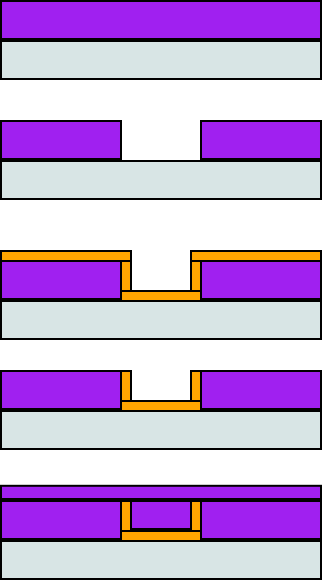
\includegraphics[scale=0.5]{images/metal-process.png}
\caption{Metalization process. Blue-gray=$Si$, purple=$SiO_2$, yellow=$Au$}
\label{metal-process}
\end{figure}
\pagebreak
